\documentclass[final,xcolor={dvipsnames,svgnames,x11names,table}]{beamer}
\usetheme{RJH}
%\usetheme{Boadilla}
\usepackage[orientation=portrait,size=a0,scale=1.3]{beamerposter}
% \usepackage[orientation=portrait, size=custom, width=84.1, height=118.9, scale=1]{beamerposter}
\usepackage[absolute,overlay]{textpos}
\usepackage{pifont}
\usepackage{ulem}
\usepackage{bm}
\usepackage{siunitx}
\usepackage[export]{adjustbox}
\usepackage{gmp}
\usepackage{smartdiagram}
\usesmartdiagramlibrary{additions}
\usepackage{booktabs}
%\usepackage{enumitem}

%\DeclareGraphicsRule{.1}{mps}{*}{}

\usepackage[listings,theorems]{tcolorbox}


\usepackage{libertine}
\setlength{\TPHorizModule}{1cm}
\setlength{\TPVertModule}{1cm}

\usepackage{tikz,tikz-3dplot} %nalipour
\usetikzlibrary{shapes,arrows, decorations.pathreplacing}%, snakes} %nalipour

\def\Put(#1,#2)#3{\leavevmode\makebox(0,0){\put(#1,#2){#3}}}

% Raised Rule Command:
%  Arg 1 (Optional) - How high to raise the rule
%  Arg 2            - Thickness of the rule
\newcommand{\raisedrule}[2][0em]{\leaders\hbox{\rule[#1]{1pt}{#2}}\hspace{13.5cm}}

\newcommand{\dotrule}[1]{%
   \parbox[]{#1}{\dotfill}}

\setbeamertemplate{bibliography entry title}{}
\setbeamertemplate{bibliography entry location}{}
\setbeamertemplate{bibliography entry note}{}
\footer{}


% \usebackgroundtemplate{%%\includegraphics[width=\paperwidth]{Figures/CLIC_canvas_accelerator_small.jpg}}


\title{\Huge{Simulation of the IDEA Drift Chamber at the FCC-ee}\vspace*{0.5cm}}
\author{\vspace*{1.5cm}{\Large{\underline{N.~Alipour~Tehrani (CERN)}, B.~Hegner, F.~Grancagnolo, P.~Janot, A.~M.~Kolano,  G.~F.~Tassielli, G.~Voutsinas}\\\vspace*{1.5cm}{\Large{2018 IEEE Nuclear Science Symposium and Medical Imaging Conference}\\ \vspace*{0.8cm}\large{10 - 17 November 2018, International Convention Center Sydney, Australia}}}}
% \footer{}
\institute{CERN}
\date{}
%\footimage{}

\usepackage[backend=bibtex]{biblatex}
\addbibresource{ref.bib}
% \setbeamertemplate{bibliography item}[text]
% \renewcommand*{\bibfont}{\footnotesize}

% tcolorbox styles
\tcbset{%
    noparskip,
    colback=white, %background color of the box
    colframe=i6colorblockbg, %color of frame and title background
    coltext=black, %color of body text
    coltitle=white, %color of title text
    fonttitle=\bfseries,
    alerted/.style={coltitle=red,
                     colframe=gray!40},
    subtcolorbox/.style={coltitle=black,
                     colframe=i6colorscheme3,
                     colback=white,
                     coltitle=i6colorblockbg},
    }


\begin{document}
\begin{frame}

\begin{textblock}{6}(0.8, 9)

\includegraphics[width=\textwidth]{Figures/logo_cern.pdf}
\end{textblock}
\begin{textblock}{10}(7, 9)

\includegraphics[width=\textwidth]{Figures/FCC-logo}
\end{textblock}
\begin{textblock}{10}(71, 9)

\includegraphics[width=\textwidth]{Figures/IEEE_logo}
\end{textblock}


%%%%%%%%%%%%%%%%%%%%%%%%%%%%%%%%%%%%%
%%% Block %%%
%%%%%%%%%%%%%%%%%%%%%%%%%%%%%%%%%%%%%
\begin{textblock}{44.5}(0.5, 16)
  \begin{tcolorbox}[title=The Future Circular Collider Experiment (FCC)]

  \begin{columns}
    \column{0.6\textwidth}
      \begin{itemize}
        \item A possibility for the post-LHC era at CERN \vspace{0.5cm}

          \begin{itemize}
            \item First step: FCC-ee (electron - positron)
            \item Ultimate goal: FCC-hh (proton - proton)
            \item Optional: FCC-eh (electron - proton) \vspace{0.5cm}
          \end{itemize}
        \item $\sim$100~km tunnel in Geneva area \vspace{0.5cm}
        \item FCC-ee collider parameters: \vspace{0.5cm}
      \end{itemize}
        \centering
      	\begin{tabular}{| l | c | c | c | c |}
        	\toprule
      	   Stages & Z & WW & H (ZH) & t\={t} \\
      	   \midrule
           Center of mass energy $\sqrt{s}$ [GeV] & 91.2 & 160 & 240 & 365 \\
           Average bunch spacing [ns] & 19.6 & 163 & 994 & 3396\\
      	   \bottomrule
      	\end{tabular}

    \vspace{0.5cm}

    \column{0.4\textwidth}
      \centering
      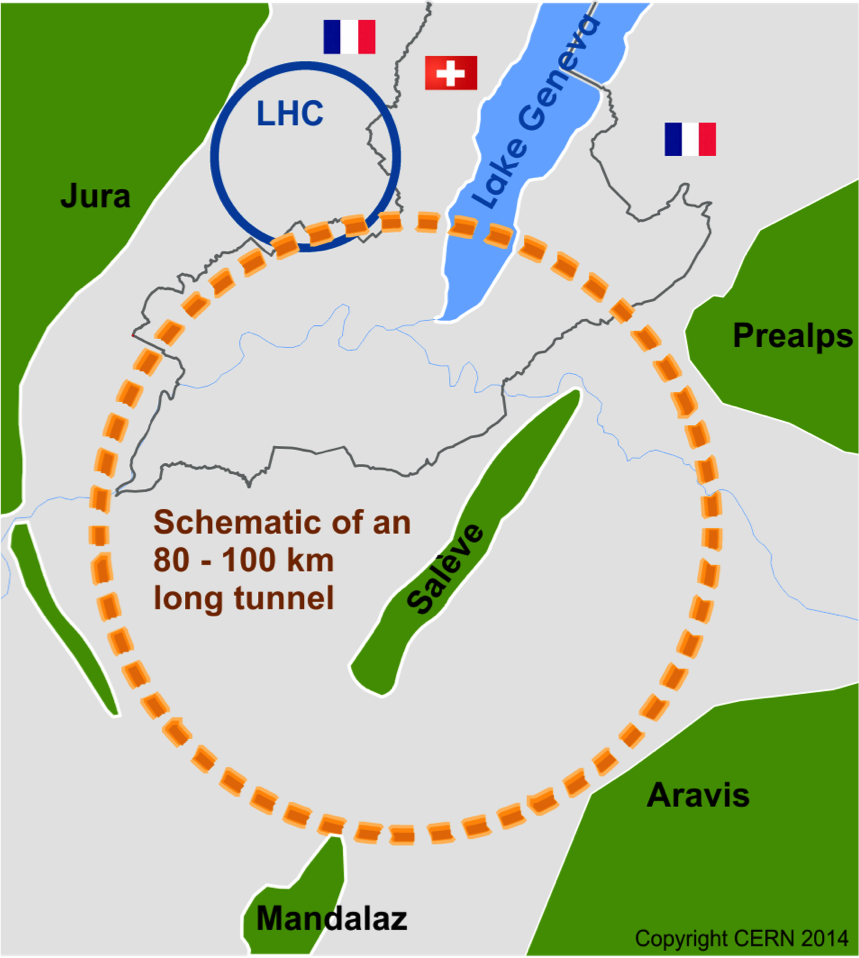
\includegraphics[width=0.9\textwidth]{Figures/cernFCC}
  \end{columns}

  \end{tcolorbox}
\end{textblock}

% %%%%%%%%%%%%%%%%%%%%%%%%%%%%%%%%%%%%%
% %%% Block %%%
% %%%%%%%%%%%%%%%%%%%%%%%%%%%%%%%%%%%%%
\begin{textblock}{38}(45.5, 16)
  \begin{tcolorbox}[title=FCCSW: simulation software for FCC]

  \vspace{0.5cm}
  \begin{itemize}
    \item Common \textsc{Geant4}-based software for all FCC experiments (ee, hh \& eh)~\cite{FCCSW} \vspace{0.5cm}
    \item Detector and physics studies \vspace{0.5cm}
      \begin{itemize}
        \item Fast \& full simulations
        \item One software stack from event generation to physics analysis \vspace{0.5cm}
      \end{itemize}
    \item Collaborative approach with other CERN experiments \vspace{0.5cm}
      \begin{itemize}
        \item Gaudi from LHC~\cite{Gaudi} $\Rightarrow$ software architecture
        \item DD4hep~\cite{DD4hep} from CLIC \& LHCb $\Rightarrow$ detector description
        \item New solutions where needed
      \end{itemize}
    \item The simulation pipeline
  \end{itemize}

  \vspace{0.5cm}

  \centering
   % \scalebox{2}{
  	 \smartdiagramset{back arrow disabled=true, module minimum width=6cm, text width=6cm, module minimum height=3cm, module x sep=8cm}
  	 	\smartdiagram[flow diagram:horizontal]
  	 	{%
  	   	{Geometry\\DDhep}, Segmentation, {\textsc{Geant4} \\simulation}, Digitization%
  	 	}
     % }
     \vspace{0.5cm}
  \end{tcolorbox}
\end{textblock}

% %%%%%%%%%%%%%%%%%%%%%%%%%%%%%%%%%%%%%
% %%%                             Block                                %%%
% %%%%%%%%%%%%%%%%%%%%%%%%%%%%%%%%%%%%%
\begin{textblock}{83}(0.5, 36)
  \begin{tcolorbox}[title=The IDEA detector concept for FCC-ee]

  \begin{columns}
    \column{0.3\textwidth}
      \begin{itemize}
        \item The IDEA detector is one of the two detector concepts for the FCC-ee \vspace{0.5cm}
        \item Main features of the IDEA concept \vspace{0.5cm}
          \begin{itemize}
            \item Vertex detector: MAPS \vspace{0.2cm}
            \item Ultra-light drift chamber with particle identification \vspace{0.2cm}
            \item Dual-readout calorimetry \vspace{0.2cm}
            \item Aditional silicon disk layers placed in the space between the drift chamber and the dual readout calorimeter to serve as a precise tracking layer and a pre showering device \vspace{0.2cm}
            \item 2~T axial magnetic field \vspace{0.2cm}
            \item Instrumented return yoke \vspace{0.2cm}
            %\item Large tracking volume (R $\sim$ 8~m) for very weakly coupled (long-lived) particles
          \end{itemize}
      \end{itemize}


    \column{0.25\textwidth}
      \centering
      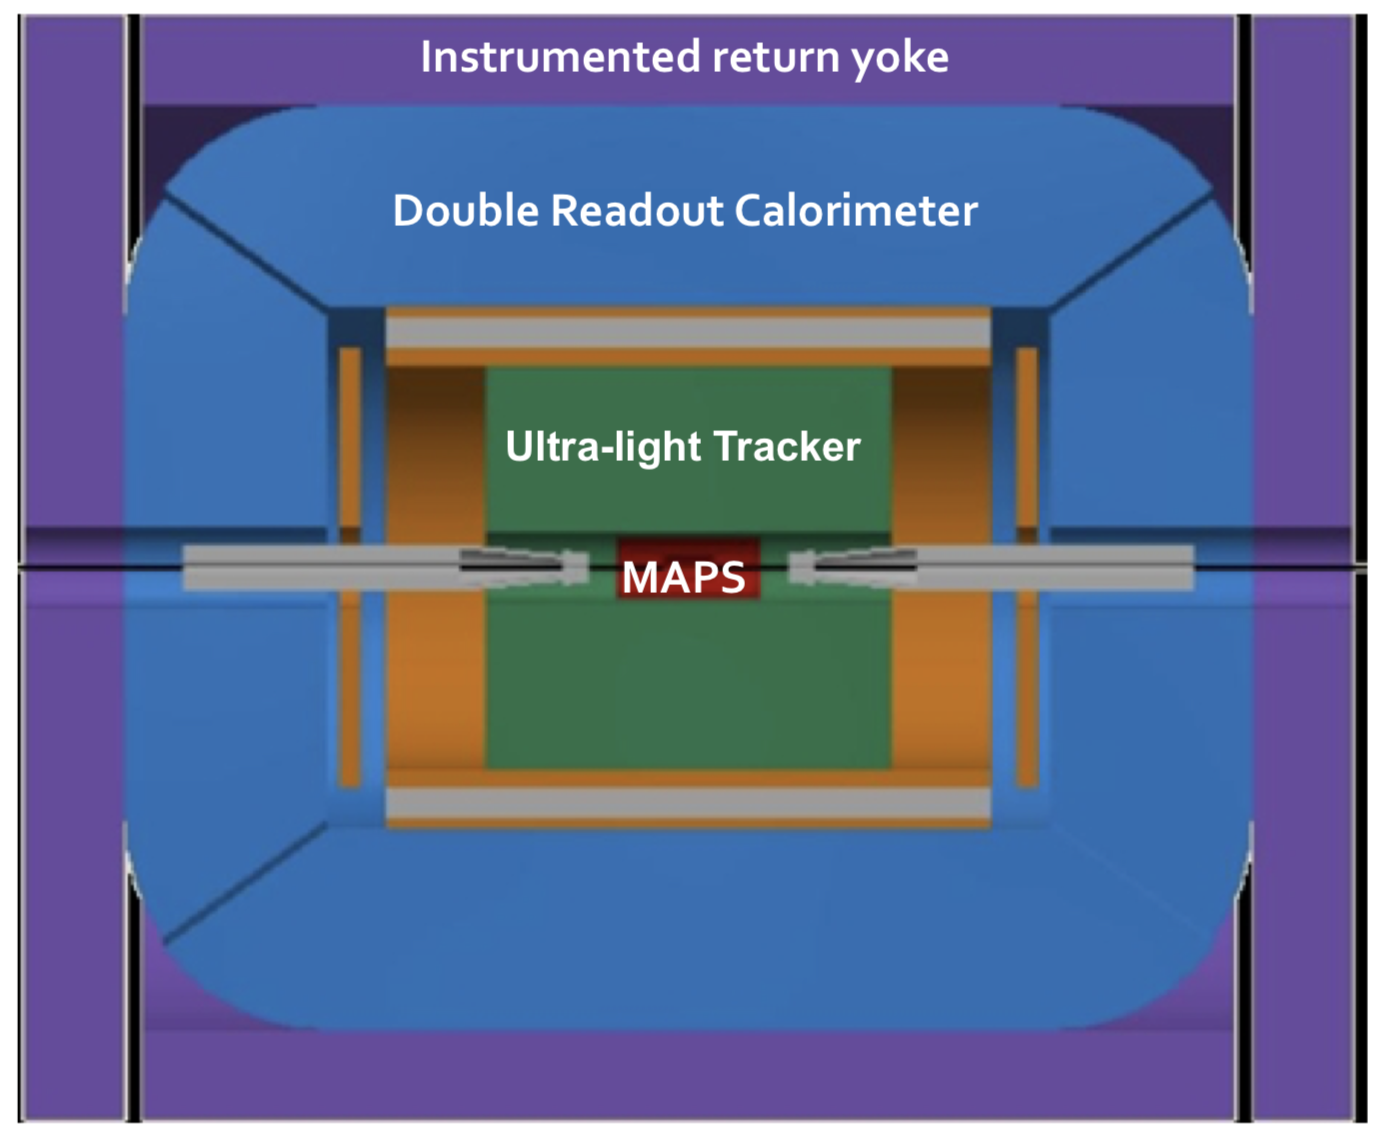
\includegraphics[width=\textwidth]{../figures/FCCeeIDEAConcept}

    \column{0.45\textwidth}

    \begin{itemize}
      \item The IDEA detector as currently simulated with FCCSW
    \end{itemize}

    \centering
    \begin{tikzpicture}
      \node[anchor=south west,inner sep=0] (image) at
      (0,0){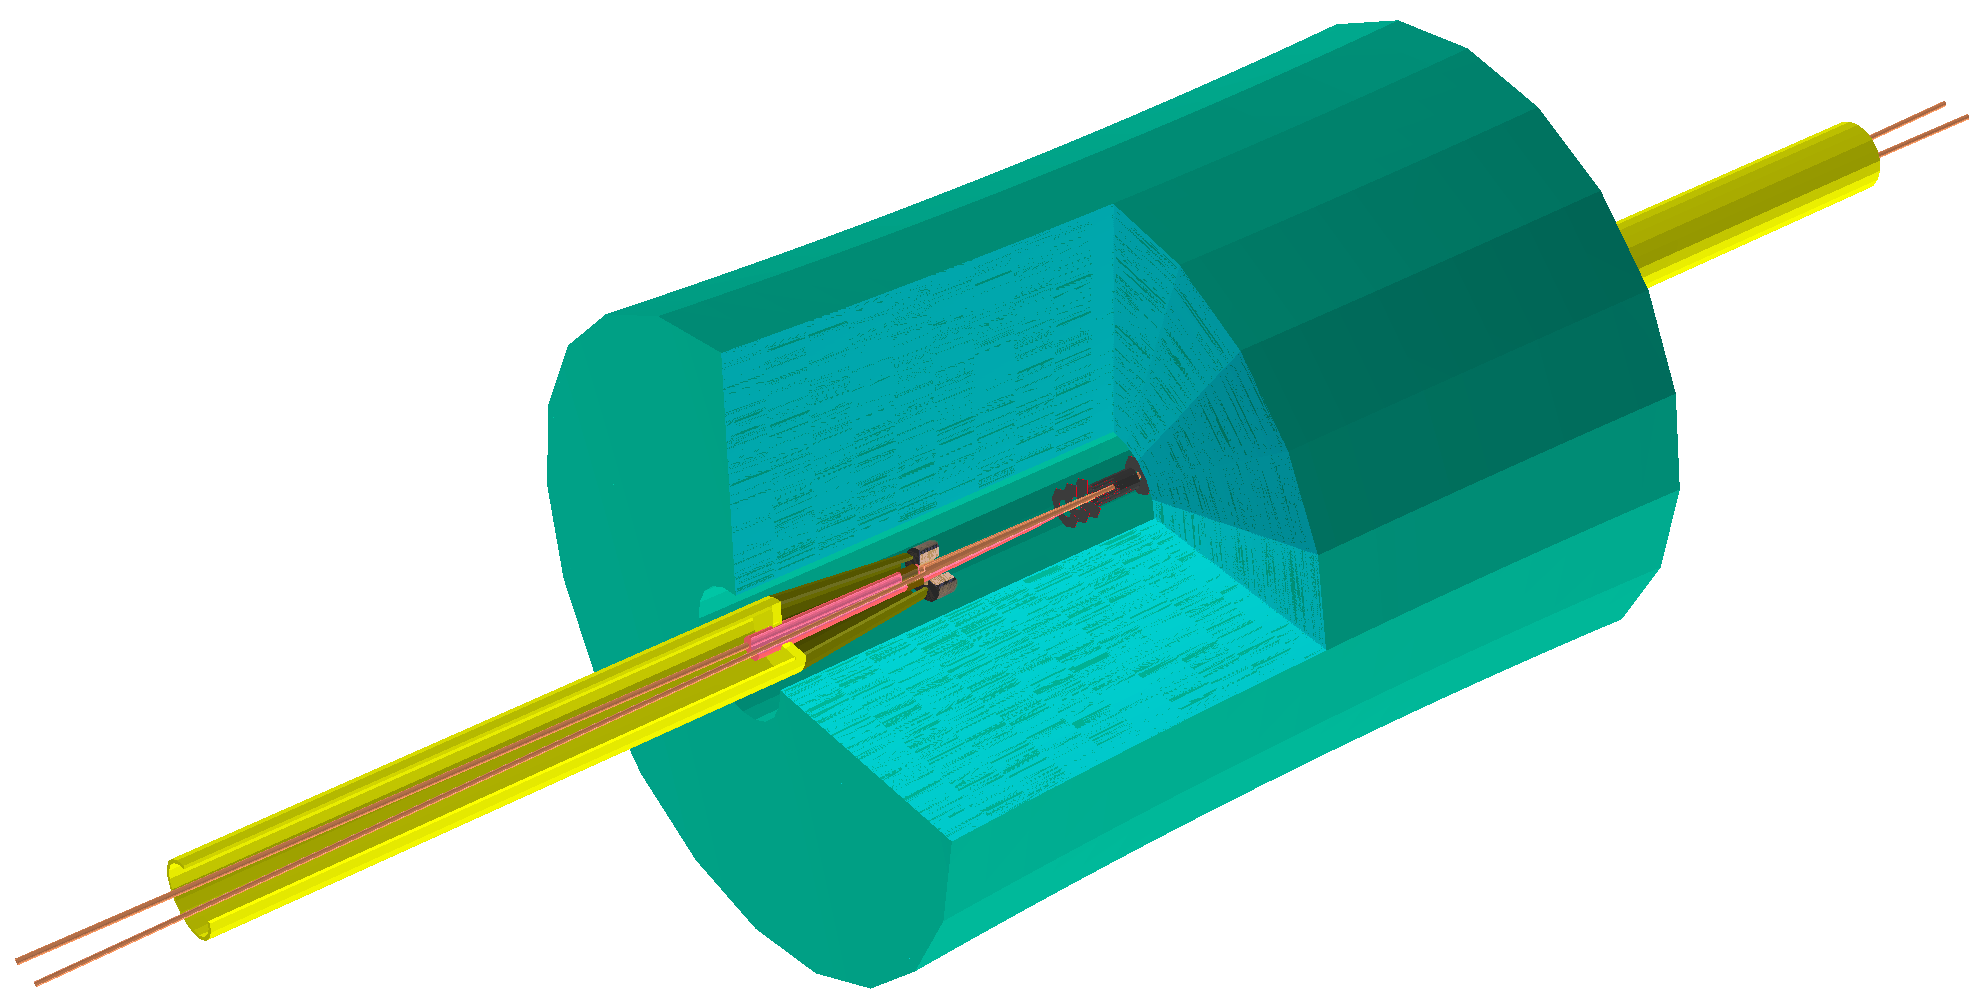
\includegraphics[width=0.9\textwidth]{Figures/FCCeeIDEA_IR}};
      \begin{scope}[x={(image.south east)},y={(image.north west)}]
      \node[left] at (0.6, 0.7) {\textbf{Drift Chamber}};

      \draw[->, thick](0.05, 0.25) -- (0.05, 0.1);
      \node[above] at (0.05, 0.25) {\textbf{Beam Pipe}};

      \draw[->, thick](0.15, 0.45) -- (0.15, 0.22);
      \node[above] at (0.15, 0.45) {\textbf{Solenoid Shielding}};

      \draw[->, thick](0.2, 0.7) -- (0.42, 0.4);
      \node[above] at (0.2, 0.7) {\textbf{Tungsten Shielding}};

      \draw[->, thick](0.55, 0.05) -- (0.48, 0.4);
      \node[below] at (0.55, 0.05) {\textbf{Luminosity Calorimeter}};

      \draw[->, thick](0.75, 0.2) -- (0.58, 0.5);
      \node[below] at (0.75, 0.2) {\textbf{Vertex Detector}};

    \end{scope}
    \end{tikzpicture}
  \end{columns}


  \end{tcolorbox}
\end{textblock}

%%%%%%%%%%%%%%%%%%%%%%%%%%%%%%%%%%%%%
%%% Block %%%
%%%%%%%%%%%%%%%%%%%%%%%%%%%%%%%%%%%%%
\begin{textblock}{43}(0.5, 58.4)
  \begin{tcolorbox}[title=The IDEA drift chamber]

    \begin{itemize}
      \item The gas volume is divided into a set of hyperboloid layers. \vspace{0.2cm}
      \item Each layer contains single sense wire cells. \vspace{0.2cm}
      \item Field wires surround the sense wires to provide homogeneous electric field for each cell. \vspace{0.2cm}
      \item The wires are rotated with an average stereo angle of 0.1~radians to improve the longitudinal resolution along them. \vspace{0.2cm}
    \end{itemize}

    \begin{columns}
    \column{0.6\textwidth}
      \begin{itemize}
        \item The parameters of the drift chamber \vspace{0.5cm}
      \end{itemize}

      \centering
      \begin{adjustbox}{max width=0.8\textwidth}
        \begin{tabular}{l l}
          \toprule
            Gas & $90~\%$ Helium \&\\
            & $10~\%$ isobutane ($\text{C}_{4}\text{H}_{10}$) \\
            Length & 4000~mm \\
            Inner radius & 345~mm \\
            Outer radius & 2000~mm\\
            Nb. layer & 112 \\
            Cell size & 12~mm - 14.7~mm \\
            Number of sensitive wires & 56448 \\
            Transverse resolution & 0.1~mm \\
            Longitudinal resolution & 1~mm \\
          \bottomrule
        \end{tabular}
      \end{adjustbox}

    \column{0.4\textwidth}
      \centering
      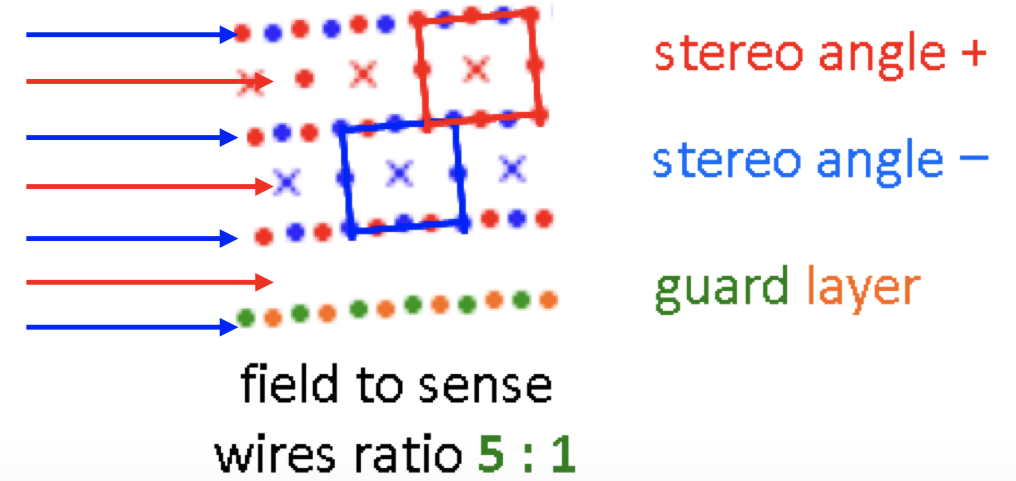
\includegraphics[width=\textwidth]{Figures/Field_sensWires.png}

    \end{columns}

  \vspace{0.5cm}

  \end{tcolorbox}
\end{textblock}


%%%%%%%%%%%%%%%%%%%%%%%%%%%%%%%%%%%%%
%%% Block %%%
%%%%%%%%%%%%%%%%%%%%%%%%%%%%%%%%%%%%%
\begin{textblock}{39.5}(44, 58.4)
  \begin{tcolorbox}[title=The simulation of the drift chamber with FCCSW]

    \begin{columns}
    \column{0.5\textwidth}
      \begin{itemize}
        \item The sensitive wires as simulated in the first layer of the drift chamber with FCCSW. \vspace{0.5cm}
        \item The DD4hep segmentation (\textsc{DDSegmentation}) is responsible to associate a hit to the wire it drifts to \vspace{0.5cm}
          \begin{itemize}
            \item Reduces the running time by avoiding to place each wire individually
          \end{itemize}
      \end{itemize}

      \column{0.5\textwidth}
        \centering
        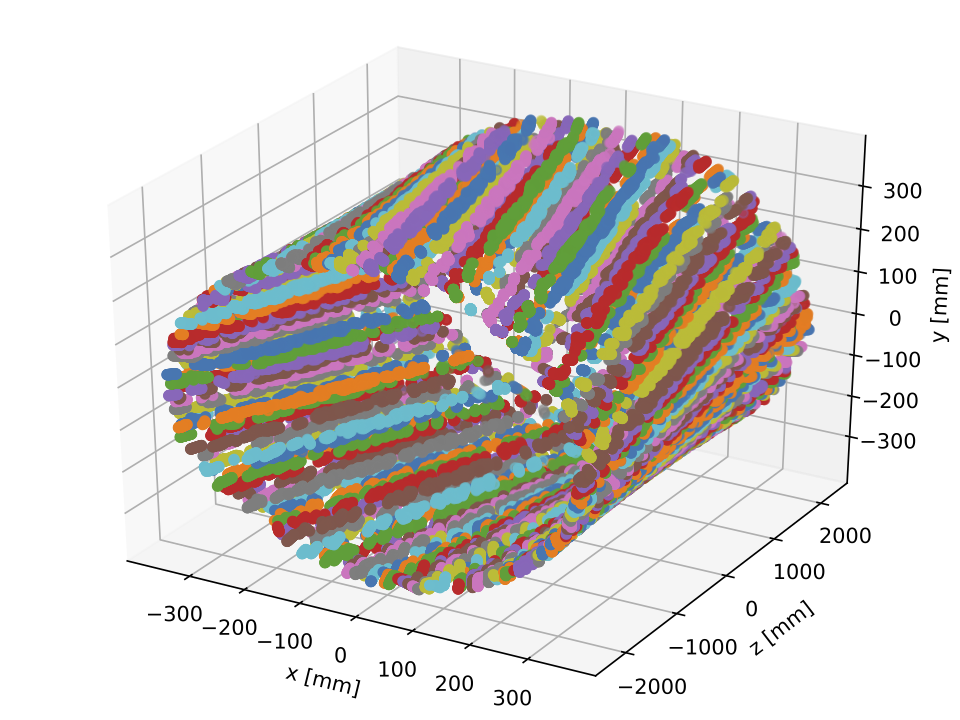
\includegraphics[width=\textwidth]{Figures/allHits}

    \end{columns}


    \begin{columns}
      \column{0.5\textwidth}
      \begin{itemize}
        \item The coverage of the drift chamber as a function of the polar angle $\theta$ is investigated using FCCSW. \vspace{0.5cm}
        \item High coverage in the barrel region by $\sim 112$ wires in average. \vspace{0.5cm}
        \item In the forward region, silicon disks are foreseen to improve the track angle coverage. \vspace{0.5cm}
      \end{itemize}

      \column{0.5\textwidth}
        \centering
        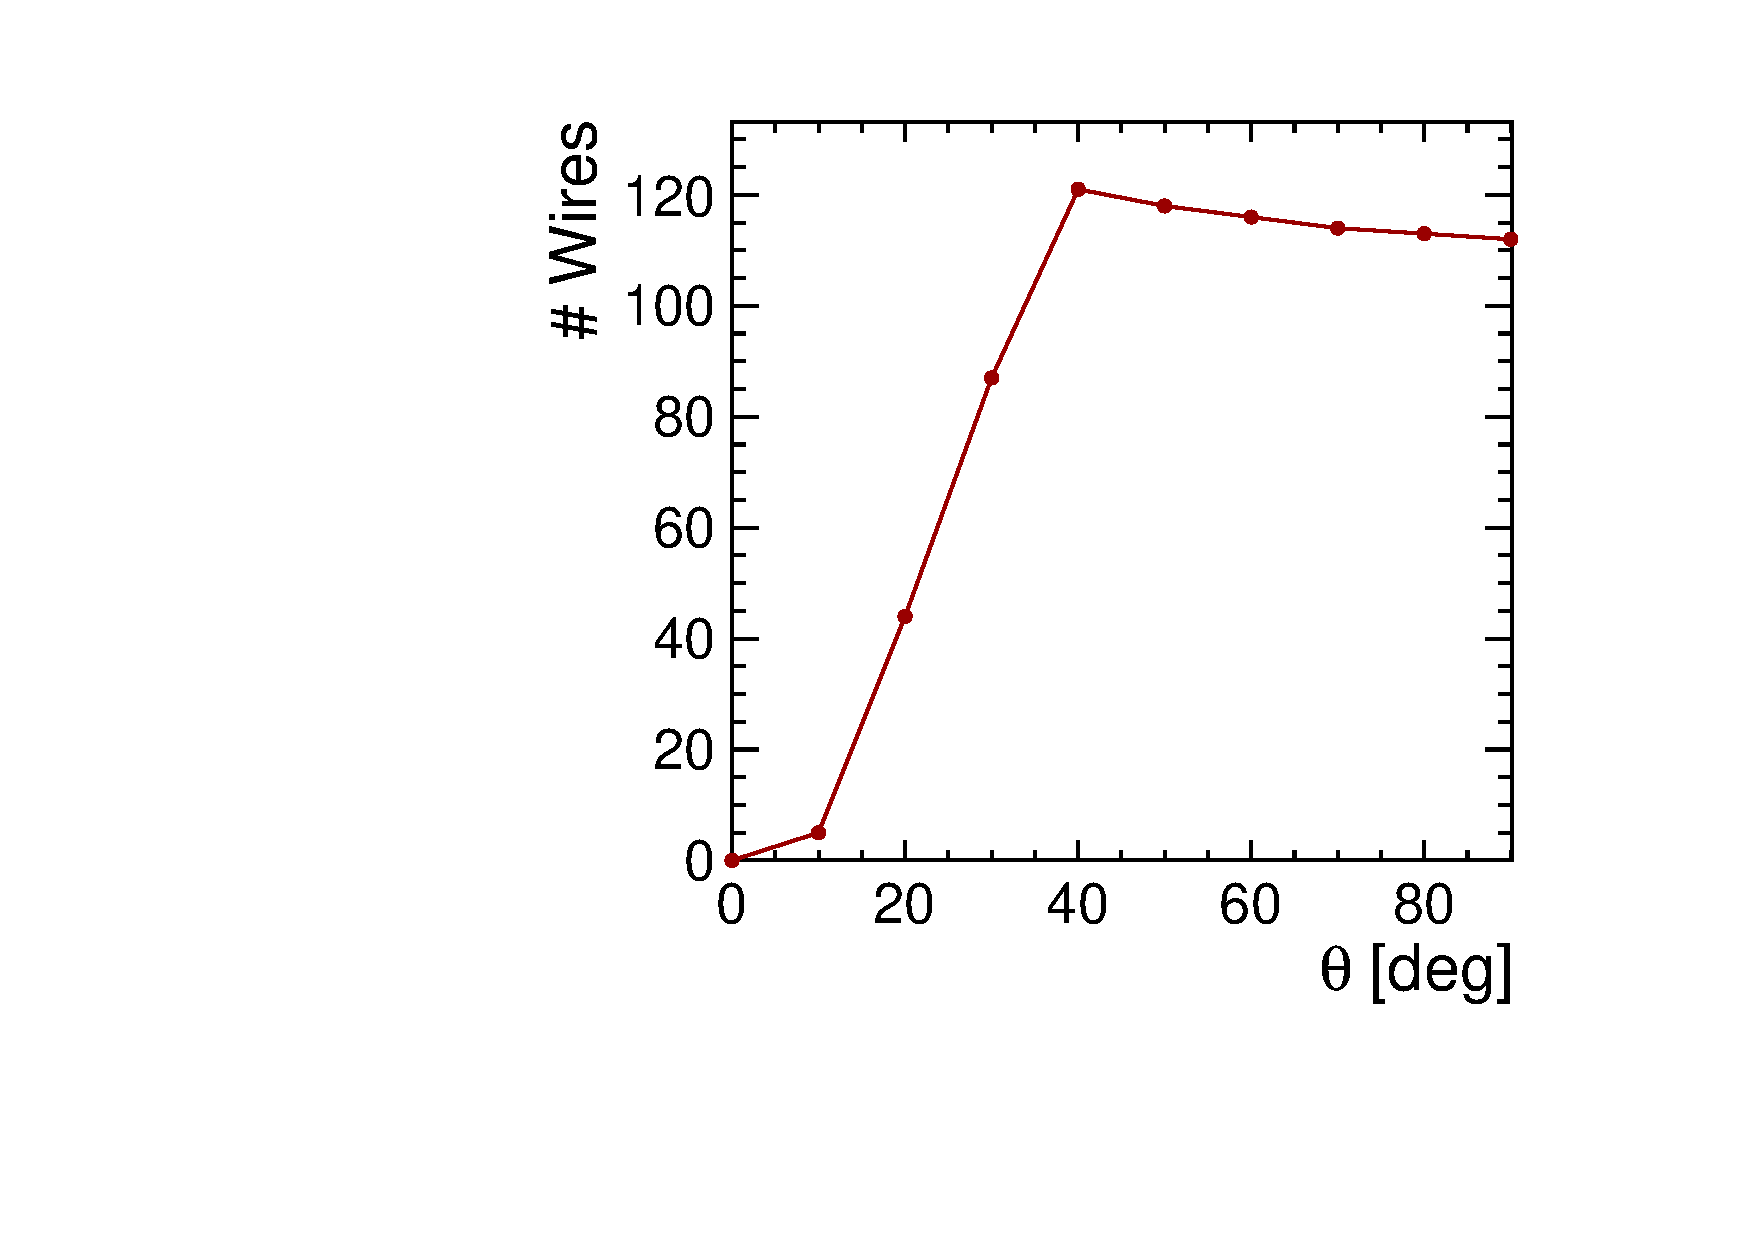
\includegraphics[width=\textwidth]{Figures/numWires}
    \end{columns}

  \end{tcolorbox}
\end{textblock}



%%%%%%%%%%%%%%%%%%%%%%%%%%%%%%%%%%%%%
%%% Block %%%
%%%%%%%%%%%%%%%%%%%%%%%%%%%%%%%%%%%%%
\begin{textblock}{43}(0.5, 84.6)
  \begin{tcolorbox}[title=Beam-induced backgrounds and the impact on the drift chamber]

  \begin{itemize}
    \item Three main sources of beam-induced backgrounds at FCC-ee \vspace{0.5cm}
    \begin{itemize}
      \item \textbf{Incoherent $e^+e^-$ pairs} due to bremstrahlung photons $\Rightarrow$ highest source of background \vspace{0.3cm}
      \item \textbf{$\gamma\gamma\rightarrow$ hadrons} $\Rightarrow$ Expected to have a very low impact \vspace{0.3cm}
      \item \textbf{Synchrotron radiation (SR)} $\Rightarrow$ Dictates the design of the interaction region (IR) \vspace{0.3cm}
        \begin{itemize}
          \item Defines the beampipe radius, the design of the shielding (in Tungesten)
          \item Mostly stopped by the shielding, few SR photons can hit the detector
        \end{itemize}
    \end{itemize}
  \end{itemize}

  \begin{columns}
    \column{0.5\textwidth}
      \begin{itemize}
        \item The trajectory of the $e^+e^−$ pairs in a 2~T magnetic field (using helix extrapolation).
      \end{itemize}
      \centering
      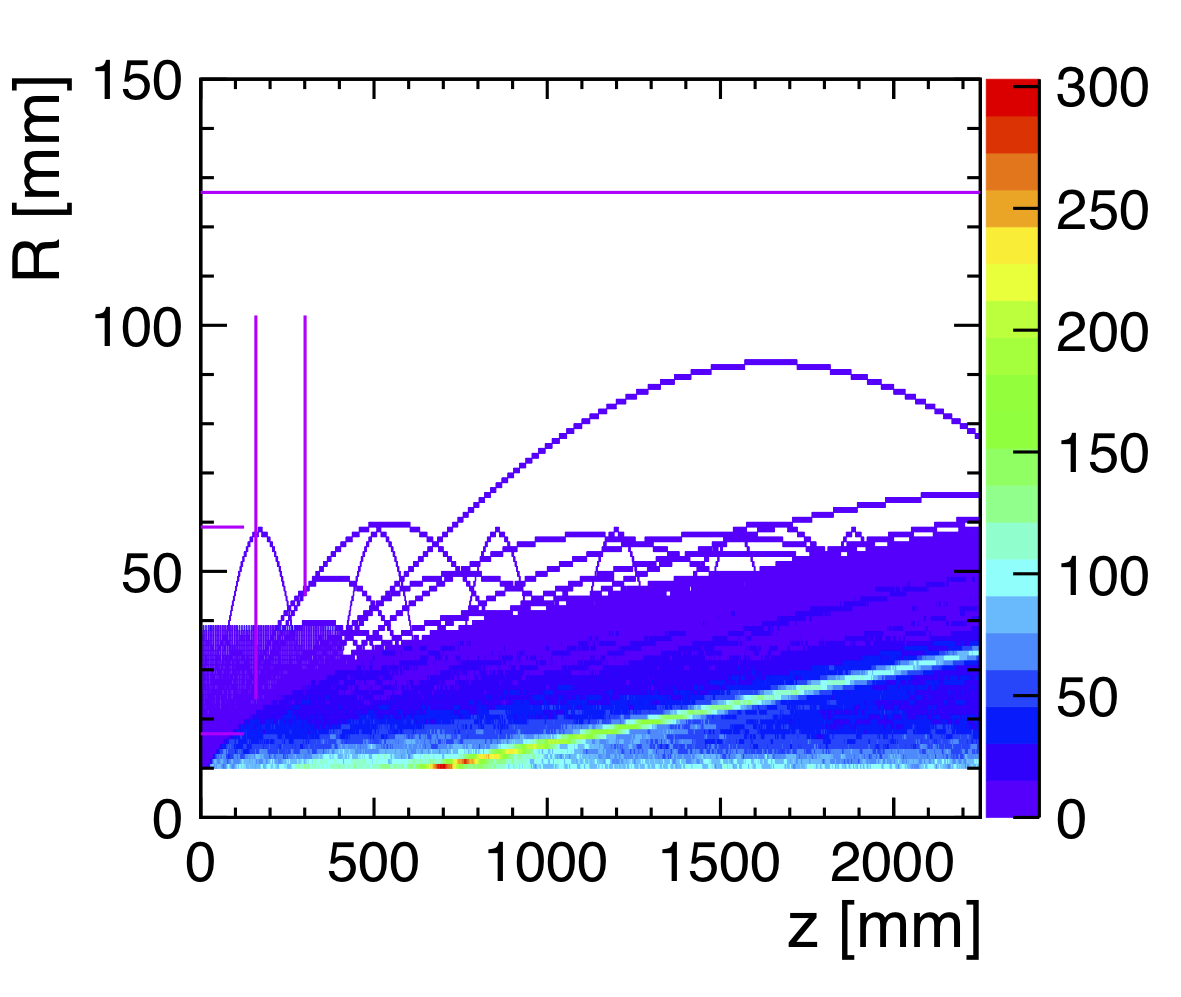
\includegraphics[width=\textwidth]{../figures/pairs_R_Z}

    \column{0.5\textwidth}

    \begin{itemize}
      \item Simulation of the hits produced in the drift chamber due to incoherent $e^+e^-$ pairs (using FCCSW)
    \end{itemize}
    \centering
    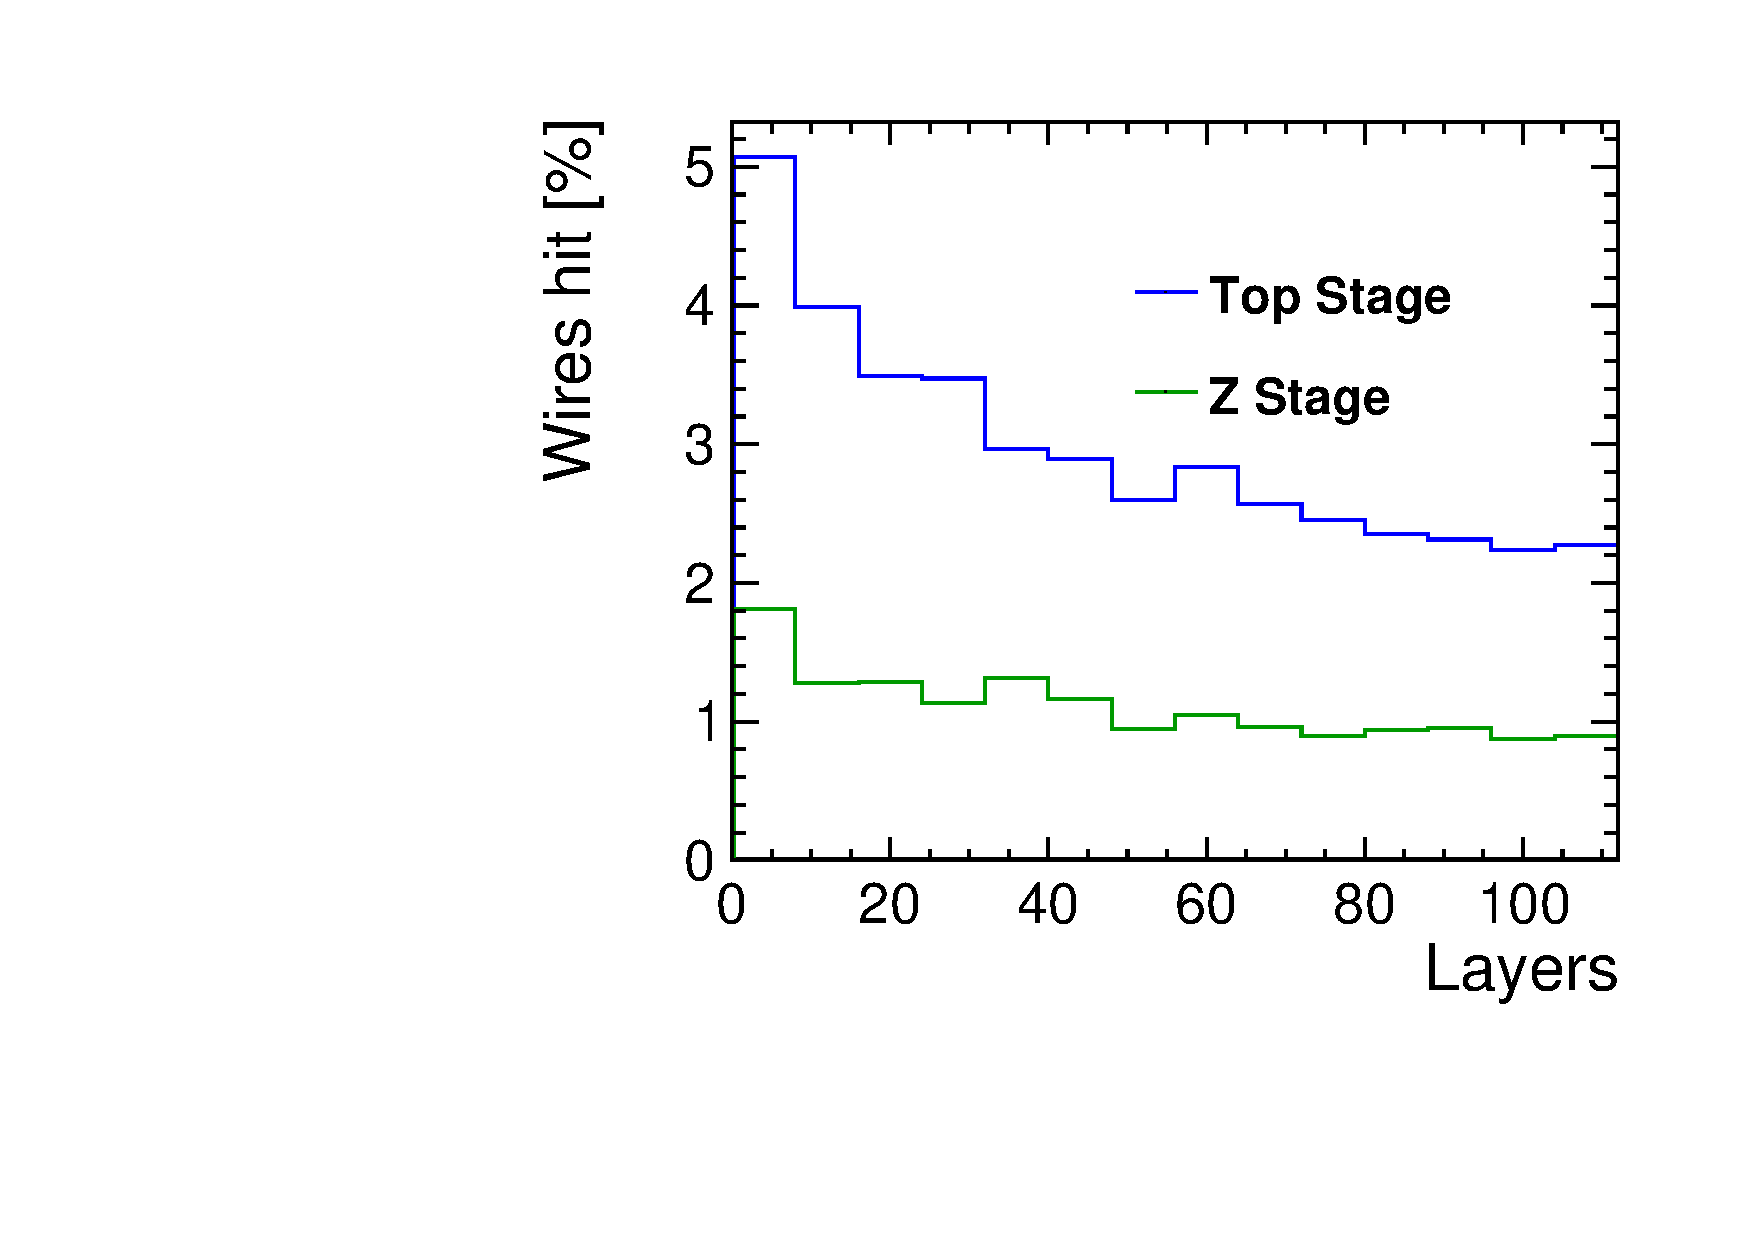
\includegraphics[width=\textwidth]{Figures/incoherent_top_Z.pdf}




  \end{columns}

  \end{tcolorbox}
\end{textblock}

% %%%%%%%%%%%%%%%%%%%%%%%%%%%%%%%%%%%%%
% %%% Block %%%
% %%%%%%%%%%%%%%%%%%%%%%%%%%%%%%%%%%%%%
 \begin{textblock}{39.5}(44, 91.3)
   \begin{tcolorbox}[title=Conclusions]

  \vspace{0.3cm}

   \begin{itemize}
     \item Summary of the occupancy of the drift chamber due to the beam-induced backgrounds \vspace{0.5cm}
   \end{itemize}
   \centering
   \begin{adjustbox}{max width=\textwidth}
     \begin{tabular}{l c c}
       \toprule
        Background & \multicolumn{2}{c}{Average occupancy} \\
         & E\textsubscript{cm} = 91.2~GeV &  E\textsubscript{cm} = 365~GeV \\
        \midrule
        $e^+e^-$ pair background & 1.1\% & 2.9\% \\
        $\gamma\gamma\rightarrow$ hadrons & 0.001\% & 0.035\%  \\
        Synchrotron radiation & - & 0.2\% \\
        \bottomrule
     \end{tabular}
   \end{adjustbox}

   \vspace{0.8cm}

   \begin{itemize}
    \item The overall impact remains low and the results are promising for the track reconstruction with this detector.
   \end{itemize}

   \vspace{0.5cm}

  \end{tcolorbox}
 \end{textblock}

% %%%%%%%%%%%%%%%%%%%%%%%%%%%%%%%%%%%%%
% %%% Block %%%
% %%%%%%%%%%%%%%%%%%%%%%%%%%%%%%%%%%%%%
 \begin{textblock}{39.5}(44, 108.5)
   \begin{tcolorbox}[title=References]

   \printbibliography

  \end{tcolorbox}
 \end{textblock}

%--------------------------------------------%
\end{frame}
\end{document}
